\documentclass[12pt]{article}
%Gummi|065|=)
\usepackage{amsmath, amsfonts, amssymb, amsfonts}
\usepackage[margin=0.5in]{geometry}
\usepackage{xcolor}
\usepackage{graphicx}

\usepackage{wrapfig}

\newcommand{\off}[1]{}
\DeclareMathSizes{20}{30}{20}{18}

\newcommand{\two }{\sqrt[3]{2}}
\newcommand{\four}{\sqrt[3]{4}}
\newcommand{\red}{\begin{tikz}[scale=0.25]
\newtheorem{thm}[subsection]{Theorem}
\draw[fill=red, color=red] (0,0)--(1,0)--(1,1)--(0,1)--cycle;\end{tikz}}
\newcommand{\blue}{\begin{tikz}[scale=0.25]
\draw[fill=blue, color=blue] (0,0)--(1,0)--(1,1)--(0,1)--cycle;\end{tikz}}
\newcommand{\green}{\begin{tikz}[scale=0.25]
\draw[fill=green, color=green] (0,0)--(1,0)--(1,1)--(0,1)--cycle;\end{tikz}}

\usepackage{tikz}

\title{Aspects of Ratner Theory}
\author{John D Mangual}
\date{}
\begin{document}

\fontfamily{qag}\selectfont \fontsize{12.5}{15}\selectfont

\maketitle

\noindent In this note we look at quantitative Ratner theory\dots the typical paradox in academica:
\begin{itemize}
\item there are techniques and results known to a few experts
\item subject hardly known outside of that clique (even among other academics)
\end{itemize} 
If you are Elon Lindenstraus or Grigory Margulis or whoever, yeah\dots you know what's going on.  \\ \\
Logically these problems are difficult because they say obvious things about common household objects. Why would you expend so much effort to prove something that's clearly true? \\ \\
Nobody told me to work on this.  Suddently I am taking on considerations like these. Here's one way into Ratner Theory.  {Legendre} proved in 1798 that:
\begin{center}
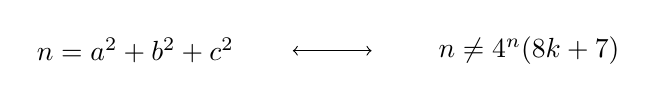
\begin{tikzpicture}  
\node at (0,0){$n = a^2 + b^2 + c^2$};
\draw[<->](2,0)--(3,0);
\node at (5,0){$n \neq 4^n(8k+7)$};
\end{tikzpicture}
\end{center}
Such a pleasant theorem.  It's quite natural to draw these thing solutions on a sphere, and all kinds of beautiful patterns emerge.  \\
\includegraphics[width=3in]{ratner-01.png}\hfill
\includegraphics[width=3in]{ratner-02.png}\\
The most natural conclusion would be these colored dots are getting evenly spread out over the ball (or sphere).  And we say the solutions to the sum of three squares problem are getting  \textit{equidistributed} as $n \to \infty$.  \\ \\
This turns out to be a very very difficult problem, only solved in 1987 by William Duke and the solution itself we very difficult to decode buried in the middle of other results.  \\ \\
Even finding one solution (instead of proving that solutions evenly spread out) is about 20 or 30 pages of algebra, that can't get shortened.

\newpage

\noindent So I think one way in this mess is to try to ask a very simple question and to try to demand a simple answer.  Let's back down a little bit:
$$ n = a^2 + b^2 + c^2 + d^2 $$
\textbf{Every positive integer is the sum of four perfect squares.} This was prove a long time ago by Lagrange.  \\ \\
These are ``solved" in the sends that a community of experts considers them solved.  Yet, I consider them open because nobody outside of that group can look inside and agree with their conclusion. \\ \\
A few more toy examples.  Here's one by Fermat about \textbf{primes as the sum of two squares}:
$$ p = a^2 + b^2 \text{ if and only if } p = 4k+1 $$
and we can ask about the angle $\theta = \tan^{-1}(\frac{b}{a})$ of the vector $(a,b) \in \mathbb{Z}^2$, and it is also evenly distribution as $p \to \infty$. If you're an expert these are pretty clear.  As a beginner, amateur, outsider whatever, these examples start to look pretty weird. \\ \\
These are my buy-ins to Ratner Theory.  The problems you look at every day, and here we put a microscope.\footnote{There should be many problems of this kind, with a basic phrasing, and a far-reaching answer.  Gradually, we'll add to this list.} \\\\\\
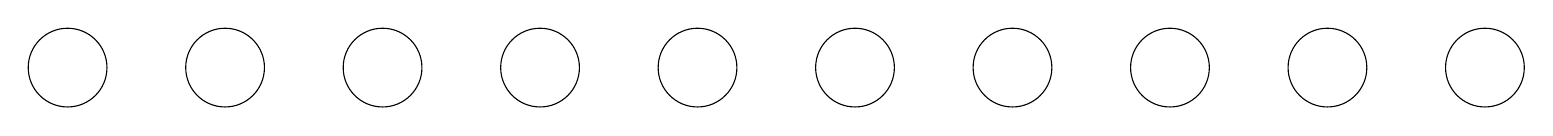
\begin{tikzpicture}
\foreach \a in {0,...,9}{
\draw (2*\a,0) circle (0.5);
}
\end{tikzpicture} \\ \\


\noindent These problems, easy to state and work on, nearly impossible to solved, are equalizers, as Erd\H{o}s would have liked. \\

\fontfamily{qag}\selectfont \fontsize{8}{10}\selectfont

\noindent The reading list is way too ambitious and there is stuff missing.  Fortunately, we're not alone.  There are always a few very smart people making headway in this way or that.  Logically, when I read the result depends on Ratner Theory, it's a signal to start over. 
There are textbooks that cover the horocycle flow or algebraic groups at just above the undergraduate level.   \\ \\
We are way ahead, because we know the result is true, but we don't know how much or by what margin.  For me the message is something like: there's no more techniques; there's you, the triangle inequality and congruences and the Pigeonhole principle.

\fontfamily{qag}\selectfont \fontsize{12.5}{15}\selectfont


\begin{thebibliography}{} 

\item Menny Aka, Manfred Einsiedler, Uri Shapira \textbf{Integer points on spheres and their orthogonal grids} \texttt{arXiv:1411.1272}

\item Manfred Einsiedler, Grigory Margulis, Amir Mohammadi, Akshay Venkatesh \textbf{Effective equidistribution and property tau} \texttt{arXiv:1503.05884}


\item Francois Dal'bo. \textbf{Geodesic and Horocyclic Trajectories} (Universitext) Springer, 2011.

\item Nicolas Bergeron. \textbf{The Spectrum of Hyperbolic Surfaces} (Universitext) Springer, 2016.



\end{thebibliography}

\newpage

\noindent \textbf{6/15}

\begin{quotation}{ \color{black!90!white}
\noindent ``\textbf{Homogeneous sets and measures} Number theoretical problems often relate to orbits of subgroups (periods) and so can be attacked
by dynamical methods\dots \\

Let~$X=\Gamma\backslash G$ be a homogeneous space defined by a lattice~$\Gamma<G$
in a locally compact group~$G$. Note that any subgroup~$H<G$ acts naturally
by right multiplication on~$X$, sending~$h\in H$ to the map~$x\in X\mapsto xh^{-1}$. 
We will refer to~$H$ as the acting subgroup.  \\ 

A {\em homogeneous (probability) measure} on $X$ is, by definition, a probability measure $\mu$ that is supported
on a single closed orbit $Y=\Gamma g H_Y$ of its stabilizer $H_Y=\mathrm{Stab}(\mu)$. 
A {\em homogeneous set} is the support of some homogeneous probability measure." }
\end{quotation}
Especially Akshay\dots the stuff he writes looks advanced.  It is very advanced, however there's always some reciprocity with material you might have learned in the very beginning (i.e. undergrad, or early graduate school). \\ \\
In a sense, you're being asked to turn away.  The paper says every good number theory problem can be turned into a dynamical systems problem:\\
\begin{center}
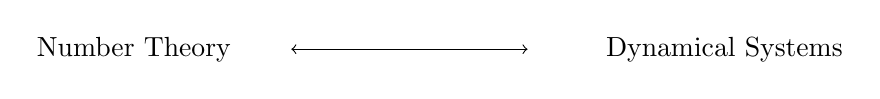
\begin{tikzpicture}
\node at (0,0) {Number Theory};
\draw[<->] (2,0)--(5,0);
\node at (7.5,0) {Dynamical Systems};
\end{tikzpicture}
\end{center}
If you read number theory literature on \texttt{arXiv}, there are a few places where dynamical systems are being mentioned, and many places where it's not being mentioned. \\\\
This example may be too old-fashioned, but it's the one I am familiar with.  Maybe it's not what they had in mind? \\
\begin{wrapfigure}{l}{0.5\linewidth}\includegraphics[width=3.5in]{primes-01.png} 
\end{wrapfigure}

\noindent Here I plotted all the solutions to $p = a^2 + b^2$ where $p = 4k+1$ is prime number.  With some effort we can show there infinitely many primes both of the $p =4k+1$ kind and also $p = 4k+3$.  The primes of the for $p = 4k+3$ cannot be written as the sum of two squares. \\ \\
I have plotted the as $(a,b)$ and also $(b,a)$ and we need to consider the signs, $(\pm a,\pm b)$ , so that the plot as been divided into octants. 
$$  \{ (a,b) : p = a^2 + b^2 \text{ and } p < N \} \times \big( \mathbb{Z}/2\mathbb{Z}\big)^3 $$
A nice artifact of this plotting strategy is an emergent circular symmetry.  Yet, the primes in $\mathbb{Z}[i]$ do not form a circularly symmetric set\footnote{The symmetry itself has to be corrected by a small error term.} \\ \\
 
\vspace{-24pt}

\noindent This problem is slightly out of date, but it was news to me.  The proof in the textbook involves L-functions and twisted by the variou ways of assigning a value to a prime number $P_{\mathbb{Z}[i]} \to \mathbb{C}$.  \\ \\ 
The proofs did not really emphasize symmetry in any way. Certainly it did not use dynamical systems or any kind of homogeneous flow.  It makes me think that maybe if I could find a good modular form, I could prove this ``Gaussian prime number theorem" in a very geometric way. \\ \\
Given Akshay's paper, maybe there's an even bigger result of the same kind.   My only complaint is they don't really prove anything too tangible.  Instead, they outline a general strategy that should work in all cases.  \\ \\
\textbf{6/16} 
\begin{quotation}

Ratner's celebrated measure classification theorem\dots ``linearization techniques"
imply in the case where $G$
is a real Lie group that, given a sequence of homogeneous probability measures
$\{\mu_i\}$ with the property that $H_i=\mathrm{Stab}(\mu_i)$ contain ``enough'' unipotents,
any weak$^*$ limit of $\{\mu_i\}$ is also homogeneous, where often
the stabilizer of the weak$^*$ limit has bigger dimension than $H_i$ for 
every $i$. \\ \\
These theorems have found many applications in number theory, but are (in most cases) ineffective. \\ \\
Our aim in this paper is  to present one instance
of an adelic result which is entirely quantitative in terms of the ``volume" of the orbits, 
and is in many cases not accessible, even in a non-quantitative form, by the measure classification theorem and linearization techniques.
A special case of this result
will recover ``property $(\tau)$'' (but with weaker exponents) from the theory of automorphic forms.
\end{quotation}
We are still reading the intro -- there's a lot being said here and a lot not being said.
\begin{itemize}
\item What was \textbf{Ratner's Theorem}?  I know it is used in one of my favorite problems, the Oppenheim Conjecture. 
\item There's a tiny bit of chaos theory, sincwe we talk about the \textbf{dimension} of of the orbit of the stabilizer.  Some of Ratner's theorems sound a bit tautological, that the the orbit has a shape with an integer dimension.  
\item What are they calling \textbf{volume}?  I think I have good geometric intuition and can understand many aspects of volume, so what are they calling volume in the space of adeles $\mathbb{A}$.
\item There's a bit of a sales-pitch.  This new theorem is so great, it's \textit{even better} than Ratner theorem (which is too diffficult anyway) so maybe their result could even be a simplification of previous results. 
\end{itemize}
There is also a shortage of examples.  I have been reluctant to write on this because I don't know enough Number Theory to really pick a group action or automorphic form.  When I read it seems like there's more but when I write I can only think of one or two.  The paper itself only gives one example about the spinor genus of quadratic forms.

\newpage

\noindent Their new theorem is rather enticing I will include their entire phrasing including some jargon:

\begin{quotation}\noindent \textbf{Theorem} [Equidistribution of adelic periods] \\\\
Let $Y_\mathcal{D}$ be a \textbf{\color{blue}{maximal algebraic semisimple homogeneous set}}
arising from $D=(\mathbf{H},\iota,g)$.
Furthermore, assume that $\mathbf{H}$ is simply connected.
Then
$$\left| \int_{Y_D}
 f \mu_D- \pi^+ f(y)\right| \ll  \mathrm{vol}(Y_D)^{-\kappa}
S(f)\quad\text{ for all } f \in C^{\infty}_c(X),$$
where $y\in Y_D$ is arbitrary, $S( f)$ denotes a certain adelic Sobolev norm,
and $\kappa$ is a positive constant which depends only on $[F:\mathbb{Q}]$ and 
$\dim \mathbb{G}$.\end{quotation}
At first glance, this result look really good.  As volume gets big, the difference is getting smaller and smaller.  There is a problem:
\begin{itemize}
\item what is a ``maximal algebraic semisimple homogeneous" (MASH) set?
\item what volume is getting bigger and bigger?  and compared to what?
\item do we have any idea of the value of $\kappa$? 
\item I barely know what a Sobolev norm is over $\mathbb{R}$ we are being askedd to define it over adeles.
\item $C_c^\infty(X)$ is compactly supported, ``smooth" functions over $X$.  What on earth does that mean over our space $X$?
\item For a given problem that I am intersted in, can we find the appropriate $G$ and $H$ ?
\end{itemize}
This is a disaster: we have no idea what they are talking about.  It sounded promising in the beginning, but maybe I have no idea how to use this framework.  Arguably, the shape of the theore is familiar and that's about it. \\ \\
However, they do give us a framework and some kind of assurance there is something like Ratner theory in the adelic setting and that it should yield an answer.\footnote{Many projects yield no answer at all\dots} \\ \\
\textbf{Long-story-short} when I take off my glasses and poke and prod, the general shape of these theorems feels extremely familiar but if I look too closely the techniques look very foreign and forbidding.  The ones we'd have to deliver upon.

\newpage

\noindent \textbf{6/17} We have exciting equidistribution results available, but there's a lot of disclaimer.  Most of their paper will be useful and we're doing a lot of the work ourselves.  And we don't have any guarantee that our problem will exactly fit Margulis' framework. \\ \\
Here is the strategy they have outlined for us:
\begin{quotation}
The dynamical argument uses {\color{red!50!yellow}unipotent flows} 
(but we note that one could also give an argument using the mixing property). 
Assuming that the volume is large, we find by a {\color{blue}pigeon-hole principle}
nearby points that have equidistributing orbits. Using {\color{purple}polynomial divergence} of the unipotent flow we obtain almost invariance under a transverse direction. By {\color{green}maximality} and {\color{green}spectral gap} on the ambient space we conclude the equidistribution.
\end{quotation}
If we need inspiration, the 4 authors have a complete discussion, or we can try to supply the details ourselves and make a comparison.  Everytime they say something abstractly, I am inclined to fill out the details.  I think that's how this paper can be read.  \\ \\
\textbf{Pigonhole principle} which I leared in 9th grade or Junior High School says that if you have more objects than spaces, the two of the must occupy the same space. 
\begin{itemize}
\item There are 400 people in a room.  Two of them have the same birthday.  \\ \\ Proof: there are 365 days i a year $<$ 400 people, so if each of 365 people had a different birthday, there are still 35 people left 
\item An softer computation show that if there are only 30 people in the room, two of them are \textit{very likely} to have the same birthday.
$$ \mathbb{P} \big( \textbf{no collision} \big) = \frac{365}{365} \times \frac{364}{365} \times \frac{363}{365} \times \dots \times \frac{365-30}{365} = \prod_{k=0}^{30} \left( 1 - \frac{k}{365}\right) 
< \prod_{k=0}^{30} e^{\frac{k}{365}} =  \exp \Big[ \frac{1}{365}\binom{30}{2} \Big] \approx \frac{1}{3}$$
The odds of two people in a room having the same birthday are \textbf{2:1} in gambling terms.
\end{itemize}
Next my image of a \textbf{unipotent flow} is the shearing of a rhombus: \\ \\
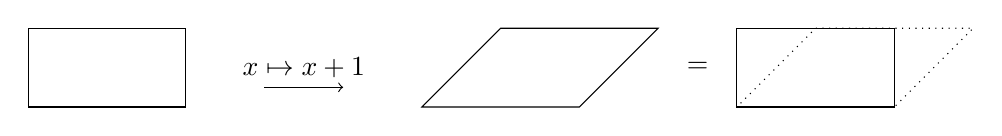
\begin{tikzpicture}

\begin{scope}
\draw (0,0)--(2,0)--(2,1)--(0,1)--cycle;
\end{scope}

\node at (3.5,0.5) {$x \mapsto x+1$};
\draw[->] (3,0.25)--(4,0.25);

\begin{scope}[xshift=5cm]
\draw (0,0)--(2,0)--(3,1)--(1,1)--cycle;
\end{scope}

\node at (8.5,0.5) {$=$};

\begin{scope}[xshift=9cm]
\draw[dotted] (0,0)--(2,0)--(3,1)--(1,1)--cycle;
\draw (0,0)--(2,0)--(2,1)--(0,1)--cycle;
\end{scope}

\end{tikzpicture} \\ 
Maybe, in Akshay and Amir's paper, the rhombus flow is happeing in a much more abstract setting over a 3-manifold $M$ or over the adel\'{e}s, $\mathbb{A}$. \\ \\
The one I understand less is \textbf{polyomial divergence}.  If I'm not mistaken one example comes out of arithmetic:
$$  1 + 2 + 3 + 4 + \dots = - \frac{1}{12}$$
which happeds because we have tried to reguarlize this sum; the left side which has no values and we're forced to assign it a number:
$$  1 \times e^{-\epsilon}+  2 \times e^{-2\epsilon} + 3 \times e^{-3\epsilon} + 4 \times e^{-4\epsilon} + \dots =  \epsilon^2 - \frac{1}{12} + O(\epsilon^2)$$
As for \textbf{maximality} I am not sure what it means;  I have no guarantee the unipotent orbit I choose will be maximal.

\newpage

\noindent The \textbf{spectral gap} is expressed rather succictly like this.  I don't know what this split means:
$$ L^2(X,\text{Vol}_G)=L^2_0(X,\text{Vol}_G)\oplus L^2(X,\text{Vol}_G)^{\mathbf{G}(\mathbb{A})^+} $$
and mixing is also going to be expressed in the language of Hilbert spaces as well:
$$ 
\Big|\int_{X\times X}
 f \, d\mu_{X_g} 
 -\int_{X\times X} f_1\otimes\bar f_2 \; d\text{Vol}_{G\times G}\Big|
 =\Big|\langle \pi_gf_1, f_2\rangle_X-
 \int_X f_1\operatorname{d}\!\text{Vol}_G\int_X\bar f_2\operatorname{d}\!\text{Vol}_G\Big|\ll 
 \|g\|^{-\kappa}\text{Sob}(f) $$
The problem is\dots all of this is so extremely speculative, it hardly makes any sense to continue.  Some parts look more familiar, and other parts I am less sure about.

\newpage

\noindent \textbf{6/19}  Time for us to pick a problem!\footnote{Venkatesh or Margulis or whowever, they give the misleading picture the algebra works out perfectly every single time.  That's what it looks like to me anyway.  \\ \\
The mess can almost be a good sign.  They are putting up a fight or whatever and but also there is room for stuff to occur.} \\ \\
There is Duke's theorem:
\begin{quotation}
\noindent For $d \to -\infty$ and $d \not \equiv 0,1,4 \pmod 8 $ the set $\mathcal{G}_d$ defined by:
$$ \mathcal{G}_d = \frac{1}{\sqrt{d}} V_{Q, |d|}(\mathbb{Z})   = \frac{1}{\sqrt{d}} 
\bigg[ (a,b,c)\in \mathbb{Z}^3: a^2 + b^2 + c^2 = d \bigg] $$
The set $\mathcal{G}_d$ is equidistributed in $S^2$ with respect to Lebesgue measure $\mu_{S^2}$.
\end{quotation}
The Lebesgue measure can assign numbers to admittedly weird sets, in counterintuitive ways.  Our plots on the first page so the answer is a type of evenness "tempered with" smaller and smaller patterns.  \\ \\
There is an \textbf{accidental isomorphism} which happens a lot in small dimensions:
$$ SO( a^2 + b^2 + c^2, \mathbb{Z}) \simeq \mathrm{PG}(B^{2, \infty})
= B^\times_{2, \infty}/ Z(B^\times_{2, \infty}) $$
This algebra notation doesn't mean much to me, but we can clarify a little bit more:
$$ (a,b,c) \in \mathbb{Q}^3 \mapsto a\,\mathbf{i} + b\,\mathbf{j} + c\,\mathbf{k} \in \mathbb{H} $$
These algebra names get a little bit annoying.  The equivalence is between  ``quadratic spaces" (which is like a metric space but with less structure, I guess)
$$ \big(\mathbb{Q}^3, Q = a^2 + b^2 + c^2 \big) \simeq \big(\mathbb{H}_{\mathrm{tr}(z) = 0} , N(z) = z \overline{z} \big) $$
We are looking for a choice of $G$ and $H$ from the first page.  Every time you solve the equation:
$$  a^2 + b^2 + c^2 = d$$
There becomes  way to embed the ring $\mathbb{Q}(\sqrt{d})$ into the quaternions:
$$ \sqrt{d} \mapsto a\,\mathbf{i} + b\,\mathbf{j} + c\,\mathbf{k}  $$
These symbols get harder and harder to look up.  It just gets more \textbf{obnoxious}. \\ \\
In the 20th century it was shown that algebra ``works" under the most general settings, but that leaves us with the problem of looking up the information we want, or conjuring up a new possibility. 
$$ \mathbf{T}_d = \mathrm{res}_{K/Q} (\mathbb{G}_m / \mathbb{G}_m ) $$
I read that the two copies of the group should cancel and therefore we should get 1:
$$ \frac{\mathbb{G}_m }{\mathbb{G}_m } = 1 $$

\newpage

\noindent Let's see $Q = a^2 + b^2 + c^2$ and $K = $
$$ \mathbf{T}_d = \mathrm{res}_{K/Q} (\mathbb{G}_m / \mathbb{G}_m ) $$
I really have better things to do with my time, then to decipher some stuck-up algebraists poorly written notations.

\end{document}